\chapter*{BIODATA PENULIS}
%*********************************
%Gambar Foto 
	\begin{center}
		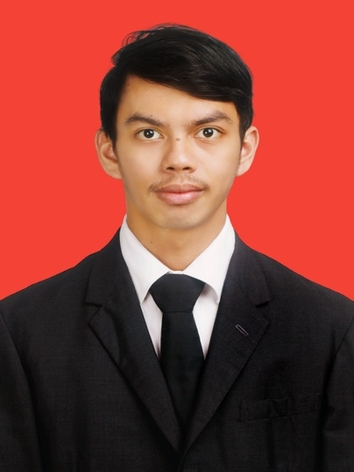
\includegraphics[height=0.2\textheight]{./ubah/3-Pas_Foto_dhani.jpg}
	\end{center}
%*********************************
\section*{Identitas Diri}
\begin{tabular}{p{3cm}cp{9cm}}
	%Masukan Identitas Disini.............
	Nama  		  & :&
		Ahmad Ramadhani \\
	Tempat Lahir  & :&
		Blitar\\
	Tanggal Lahir &:& 
		20 Desember 1998\\
	Alamat        &:& 
	Jalan Klayatan 3 Gang Teratai No. 16C RT 05 RW 02, Kelurahan Bandungrejosari, Kecamatan Sukun, Kota Malang.\\
	Email   &:&
		 ahmadramadhani2098@gmail.com\\
\end{tabular}

\section*{Riwayat Pendidikan}
\begin{tabular}{p{3cm}cp{9cm}}
	2022-Sekarang  	& :&
		Program Magister (S2), Bidang Jaringan Cerdas
		Multimedia (JCM), Departemen Teknik Elektro,
		Fakultas Teknologi Elektro dan Informatika Cerdas, Institut Teknologi Sepuluh Nopember\\
	&&\\
	2017-2021  & :&
		Program Sarjana (S1), Program Studi Pendidikan Teknik Informatika, Departemen Teknik  Elektro dan Informatika, Fakultas Teknik, Universitas Negeri Malang\\
%	&&\\
%	2014-2017  & :&
%		Program Sarjana (S1), Departemen Teknik  Elektro, Fakultas Teknologi Elektro dan Informatika Cerdas, Institut Teknologi  Sepuluh Nopember\\
%	&&\\
%	0000-0000  & :&
%		Pendidikan 1\\
%	&&\\
%	0000-0000  & :&
%		Pendidikan 2\\
%	&&\\
%	0000-0000  & :&
%		Pendidikan 3\\
\end{tabular}


\section*{Daftar Publikasi}

\begin{enumerate}
	\item A. Ramadhani, I. K. Eddy Purnama, E. Mulyanto Yuniarno and J.
	Nugroho, ”Thrombus 
	Segmentation in Ultrasound Deep Vein 
	Thrombosis (DVT) Images using 
	VGG16 and UNet based on Denoising 
	Filters,” 2023 3rd International 
	Biomedical Instrumentation and 
	Technology Conference (IBITeC) 
	2023. Universitas Islam Indonesia, 
	Yogyakarta.
	\item . S. Batan, E. M. Yuniarno, M. H. Purnomo and A. Ramadhani, "Calorie Burn Estimator on Stationary Bike using Human Body Pose Detector," 2023 International Seminar on Intelligent Technology and Its Applications (ISITIA), Surabaya, Indonesia, 2023, pp. 125-129, doi: 10.1109/ISITIA59021.2023.10221128.
	\item I. K. Sari, H. A. Rosyid, T. Prianto, S. Sanjaya and A. Ramadhani, "Non-Intrusive Laboratory Attendance Confirmation via Object Detection using YOLO," 2021 7th International Conference on Electrical, Electronics and Information Engineering (ICEEIE), Malang, Indonesia, 2021, pp. 426-430, doi: 10.1109/ICEEIE52663.2021.9616940.
	
	
%\end{enumerate}
%
%\section*{Riwayat Penelitian}
%\begin{enumerate}
%	\item \lipsum[3]
%	\item \lipsum[3]
%	\item Penelitian Ke Tiga 
%	\item Penelitian Ke Empat 
%\end{enumerate}
%\section*{Riwayat Lainnya}
%
%\lipsum[1]